The baseline for our evaluation is RocksDB -- a mature and widely-used industrial KV-store. 
\remove{RocksDB is used as storage layer of multiple popular SQL and NoSQL databases, e.g., MyRocks~\cite{MyRocks} (incarnation of MySQL) 
and MongoRocks~\cite{MongoRocks} (incarnation of MongoDB). RocksDB is an LSM-tree that is highly optimized for both read and write scenarios. 
For example, its compaction scheduling policies are highly tuned to minimize impact on mainstream data access.} 
We use the most recent RocksDB release 5.17.2, available Oct 24, 2018.  
It is worth noting that RocksDB's performance has significantly improved  over the last two years, primarily through 
optimized LSM compaction algorithms~\cite{CallaghanCompaction}.   We also compare against PebblesDB, 
a research LSM tree prototype that reduces  write amplification  and demonstrated performance advantages
over RocksDB in some scenarios~\cite{PebblesDB}. We further attempted to experiment with TokuDB~\cite{TokuDB} -- 
the only publicly available KV-store whose design is inspired by B$^\epsilon$-trees. However, TokuDB crashed 
in all executions with more than one thread, and in all single-threaded executions its performance was 
inferior to \sys's, hence these results are not presented.

% hardcoded subsections symbol since didn't have time to hack cref...
The experiment setup is described in~\S\ref{ssec:setup}. 
Performance results for \sys\ and RocksDB are presented in~\S\ref{ssec:prod} (production data)
and~\S\ref{ssec:synthetic} (synthetic data). We study  \sys's scalability and sensitivity to  
configuration settings in~\S\ref{ssec:drill}. Finally,~\S\ref{ssec:pebbles} compares \sys\ with PebblesDB.
%\cref{ssec:recover} evaluates its recovery mechanism. 
 
\subsection{Setup}
\label{ssec:setup} 

\paragraph{Testbed.} We employ a C++ implementation~\cite{Cpp-YCSB} of YCSB~\cite{YCSB}, the  de facto standard  
benchmarking platform for KV-stores. YCSB provides a set of APIs and a synthetic workload suite inspired 
by real-life applications. \inred{In order to exercise production workloads, we extend YCSB to replay log files.}
 
% Most modern KV-stores implement  YCSB adapter API's. 
%The platform decouples data access from workload generation, 
%thereby providing common ground for backend comparison. 

A typical YCSB experiment stress-tests the backend KV-store through a pool of concurrent worker threads that drive identical
(synthetic or real) workloads. A synthetic workload is defined by  (1) the ratios of get, put, and scan accesses, and 
(2) a distribution of key access frequencies. 

Our hardware is a 12-core Intel Xeon 5 machine with 4TB SSD disk. Unless otherwise stated, the YCSB driver  
exercises 12 workers. In order to guarantee fair memory allocation across KV-stores, 
we run each experiment within a Linux container with 16GB RAM. 

\paragraph{Metrics.} Our primary performance metrics are \emph{throughput} 
and \emph{latency percentiles}, as produced by YCSB. 
In addition, we measure \emph{write amplification}, namely, bytes written to storage over bytes passed from the application. 
%In order to explain the results, we also explore \emph{read amplification} (in terms of bytes as well as number of system calls per application read).  
%as well as the number of read \inred{ and write} system calls. 
%The OS performance counters are retrieved from the Linux proc filesystem. 

\paragraph{Methodology.} 
%To make sure that the results  are reproduced, 
We run 5 experiments for each data point and present the median measurement. Since experiments are long, the results vary 
little across runs. In all of our experiments, the STD was within $6.1\%$ of the mean, and in most of them below $3\%$. 
%To avoid cluttering the plots, we do not present the STD. 

\paragraph{Configuration.} 
\inred{
All experiments in~\S\ref{ssec:synthetic}, \S\ref{ssec:prod} and~\S\ref{ssec:pebbles} use the default \sys, RocksDB, 
and PebblesDB configurations, to avoid over-tuning. RocksDB's configuration the same as exercised by the public 
performance benchmarks~\cite{RocksDBPerf}. \S\ref{ssec:drill} explores different \sys\/ configurations and provides 
insights on parameter choices. We also follow the RocksDB performance guide~\cite{RocksDBMemoryTuning} to tune 
its memory resources; the results do not affect our conclusions significantly.  Finally, the PebblesDB code includes a fix 
to  a data race reported in the project's repository~\cite{pebbles-git-issue}. }

\sys's default configuration 
allocates 8GB to munks and 4GB to the row cache,
so together they consume 12GB out of the 16GB container. 
The row cache consists of three hash tables.  
The Bloom filters for funks are partitioned 16-way.  
We set the \sys\/ maximum chunk size limit to 10MB, and the rebalance size trigger to 7MB. 
The funk log size limit is 2MB for munk-less chunks, and 20MB for chunks with munks. 
Finally, we focus on the asynchronous logging mode (with synchronous logging the system
is approximately 10x slower, trivializing the results of scenarios that include puts). 
% \inred{for write intensive workloads, and 512KB for other workloads.}

\subsection{Production benchmarks}
\label{ssec:prod}
\inred{
We evaluate a prototype application that ingests and analyzes a time-series stream of mobile 
app events. We use a log of production mobile analytics engine as data source. The log captures 
a stream that generates approximately 64GB data (80M events) per minute. The events are imported 
into a table ordered by lexicographically by app id and timestamp. As described in~\S\ref{sec:intro}, 
the app id distribution is heavy-tailed, i.e., the data organization is spatially local. 

Two workloads are exercised.  

\paragraph{Put-only (data ingestion).} We load 64GB, 128GB and 256GB of data, in timestamp order. 
Figure~\ref{fig:prod:ingestion:a} depicts the ingestion rates. \sys's advantage gets more pronounced with the dataset's growth. 
For example, it ingests 256GB of data within 1.1 hours, whereas RocksDB requires 4.8 hours (4.4x speedup). 
Figure~\ref{fig:prod:ingestion:b} depicts the ingestion rate dynamics with the 256GB dataset. Although RocksDB's 
throughput is stable overall, it suffers from long periods (1min or longer) of degraded performance (10\% of the average rate), 
due to compactions. \sys's throughput is much noisier, due to frequent munk rebalances; however, it prevails even at its slowest. 
Figure~\ref{fig:prod:ingestion:c} presents the write amplification results. While \sys's write amplification is hardly affected by 
the dataset size, RocksDB's deteriorates as the dataset (and consequently, the number of LSM levels) grows. For instance, 
RocksDB's amplification factor for 256G is 11.4x, whereas \sys's is only 2.6x. 

All in all, \sys\/ is CPU-bound, whereas RocksDB is IO-bound. With 256GB data, 
e.g., \sys\/ utilizes 3x more CPU cycles, whereas RocksDB reads and writes 4x more bytes.

\paragraph{Scan-dominated (analytics).} We run on top of the KV-store produced by the ingestion 
workload. Here, 95\% of the operations are range queries, whereas the rest are puts (lagging data or fixes).  
Every range query scans a sequence of recent events within one app (i.e., all the scanned rows share 
the same app id key prefix).  We study short, medium, and long scans -- 1s, 10s, and 1min of the app's 
event history. The app id is sampled from the data distribution (i.e., popular apps are queried more frequently).  

Figure~\ref{fig:prod:analytics} depicts the throughput dynamics for the 256GB dataset with 1min queries. 
\sys's performance stabilizes almost instantly upon the transition from ingestion to analytics. This happens 
because the two workloads are identically distributed, and hence, the working set munks are already in memory, 
organized to serve the scans. It takes RocksDB almost 40 minutes to match \sys's performance. During this period, 
it goes through multiple compactions, which degrade the application throughput by 70\% on average. Eventually, 
RocksDB completes this process, populates its read cache with the working set, and catches up with \sys.
}

\begin{figure*}[tb]
\centering
\begin{subfigure}{0.33\linewidth}
%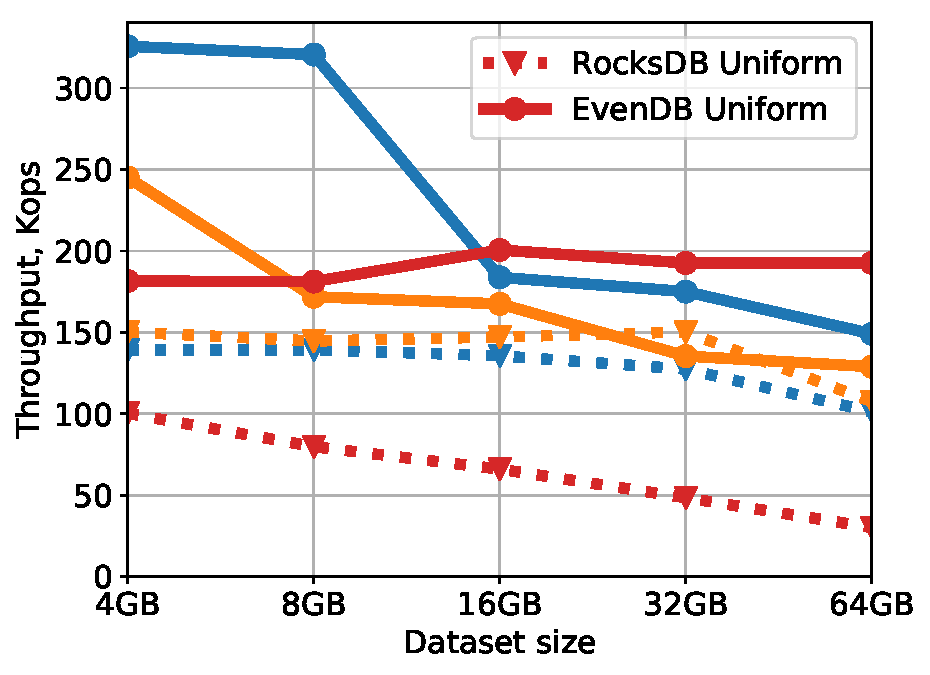
\includegraphics[width=\textwidth]{figs/Workload_P_line.pdf}
\caption{Throughput}
\label{fig:prod:ingestion:a}
\end{subfigure}
\begin{subfigure}{0.33\linewidth}
%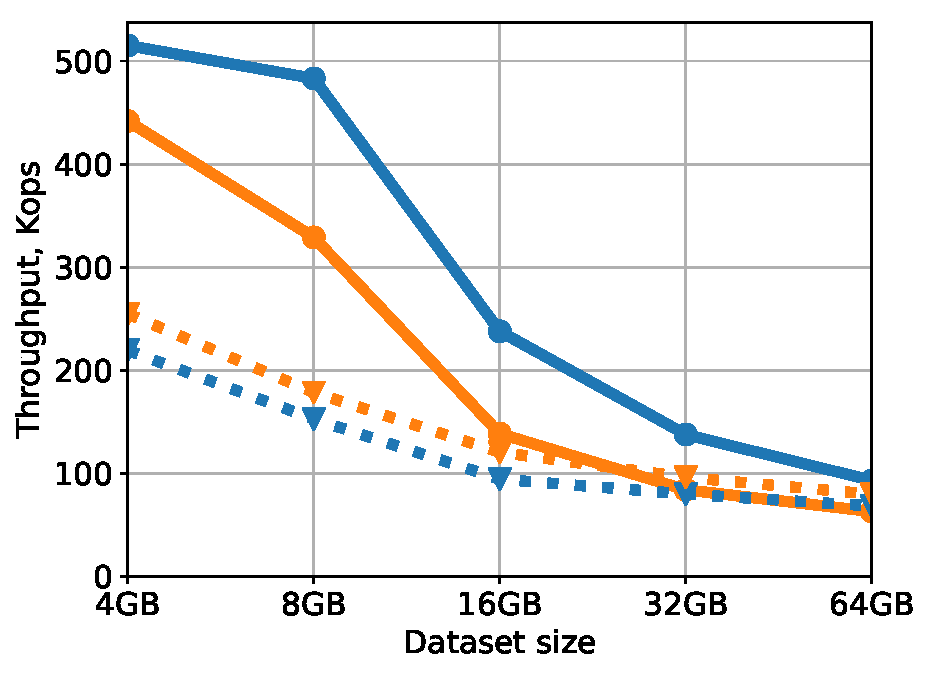
\includegraphics[width=\textwidth]{figs/Workload_A_line.pdf}
\caption{Throughput dynamics, 256GB}
\label{fig:prod:ingestion:b}
\end{subfigure}
\begin{subfigure}{0.33\linewidth}
%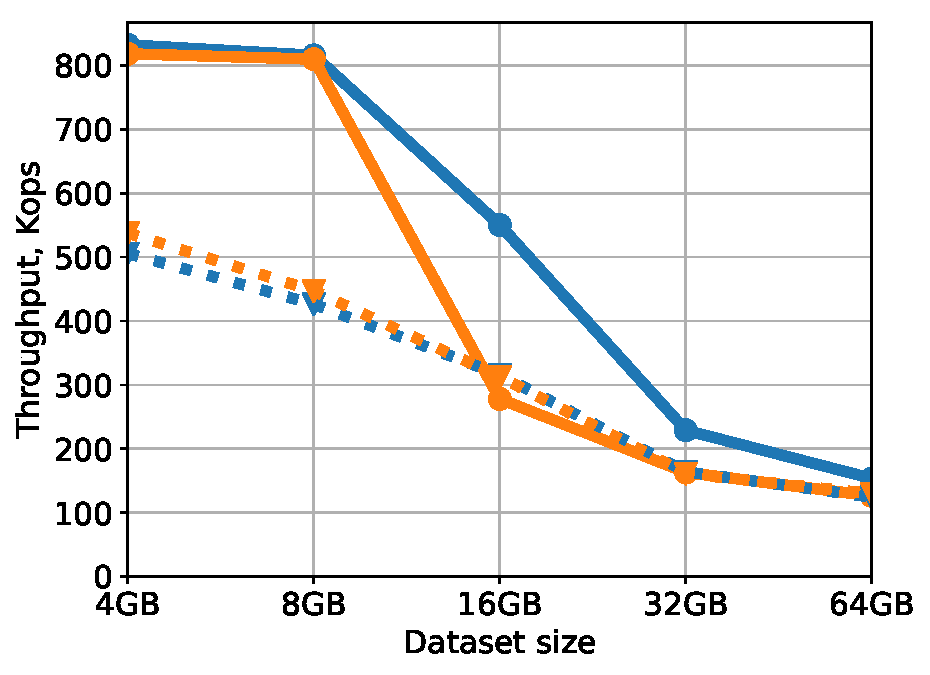
\includegraphics[width=\textwidth]{figs/Workload_B_line.pdf}
\caption{Write amplification}
\label{fig:prod:ingestion:c}
\end{subfigure}
\caption{\sys\/ vs RocksDB ingestion performance, under production workload.}
\label{fig:prod:ingestion}
\end{figure*}

\subsection{Synthetic benchmarks}
%\subsection{\sys\ versus \ RocksDB}
\label{ssec:synthetic} 

\begin{figure*}[tb]
\centering
\begin{subfigure}{0.33\linewidth}
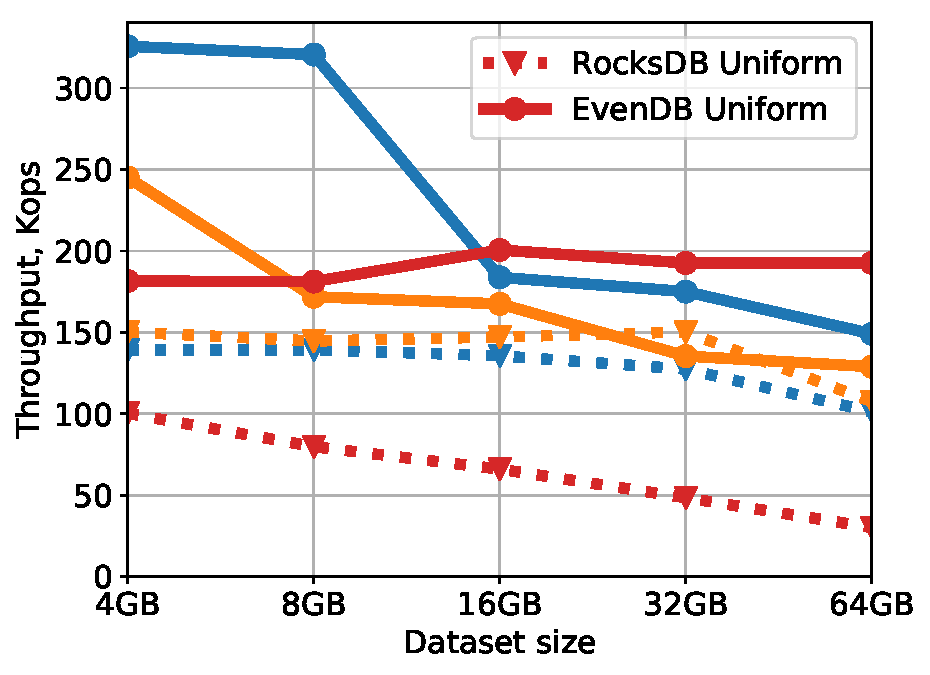
\includegraphics[width=\textwidth]{figs/Workload_P_line.pdf}
\caption{P -- 100\% put}
\label{fig:throughput:p}
\end{subfigure}
\begin{subfigure}{0.33\linewidth}
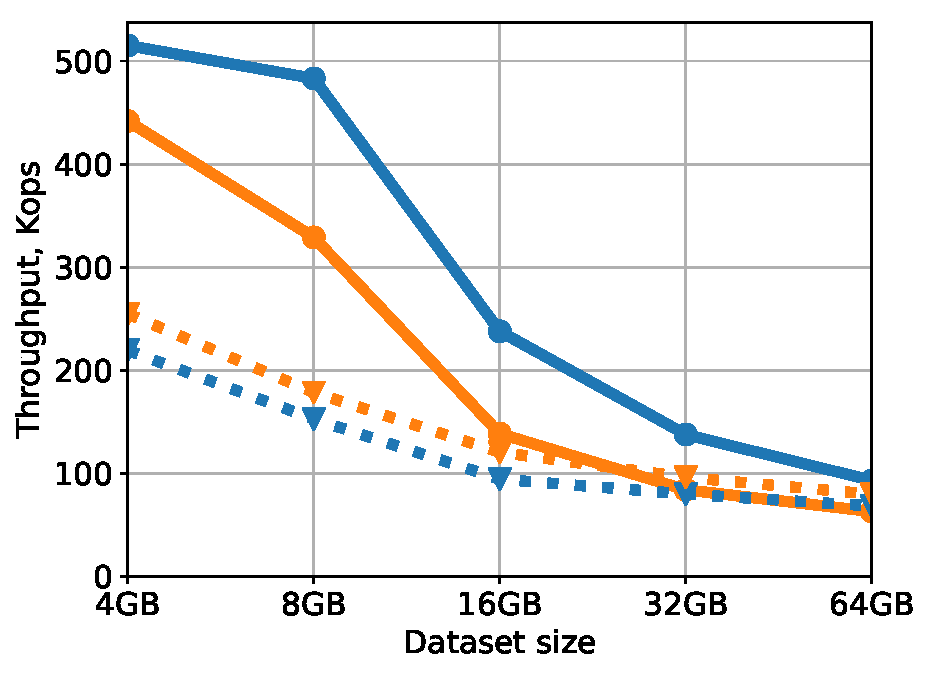
\includegraphics[width=\textwidth]{figs/Workload_A_line.pdf}
\caption{A -- 50\% put, 50\% get}
\label{fig:throughput:a}
\end{subfigure}
\begin{subfigure}{0.33\linewidth}
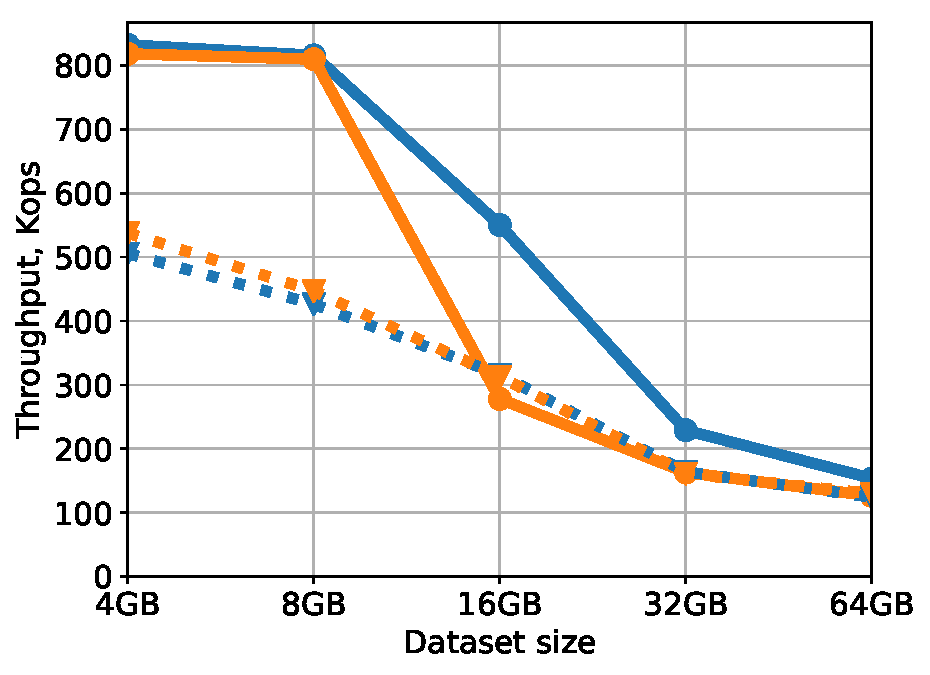
\includegraphics[width=\textwidth]{figs/Workload_B_line.pdf}
\caption{B -- 5\% put, 95\% get}
\label{fig:throughput:b}
\end{subfigure}
\hspace{70pt}
\begin{subfigure}{0.33\linewidth}
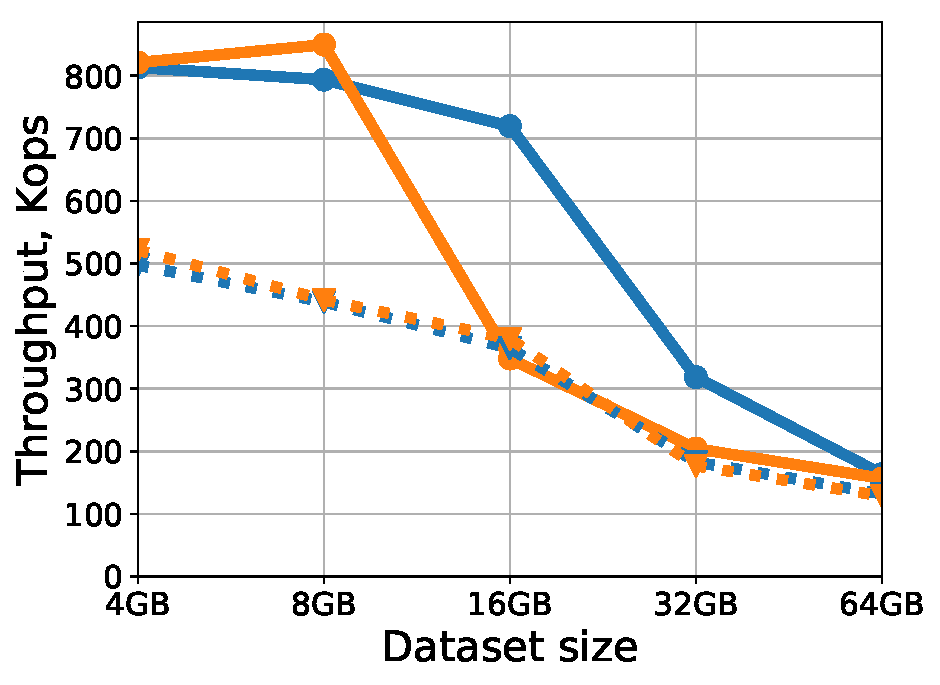
\includegraphics[width=\textwidth]{figs/Workload_C_line.pdf}
\caption{C -- 100\% get}
\label{fig:throughput:c}
\end{subfigure}
\begin{subfigure}{0.33\linewidth}
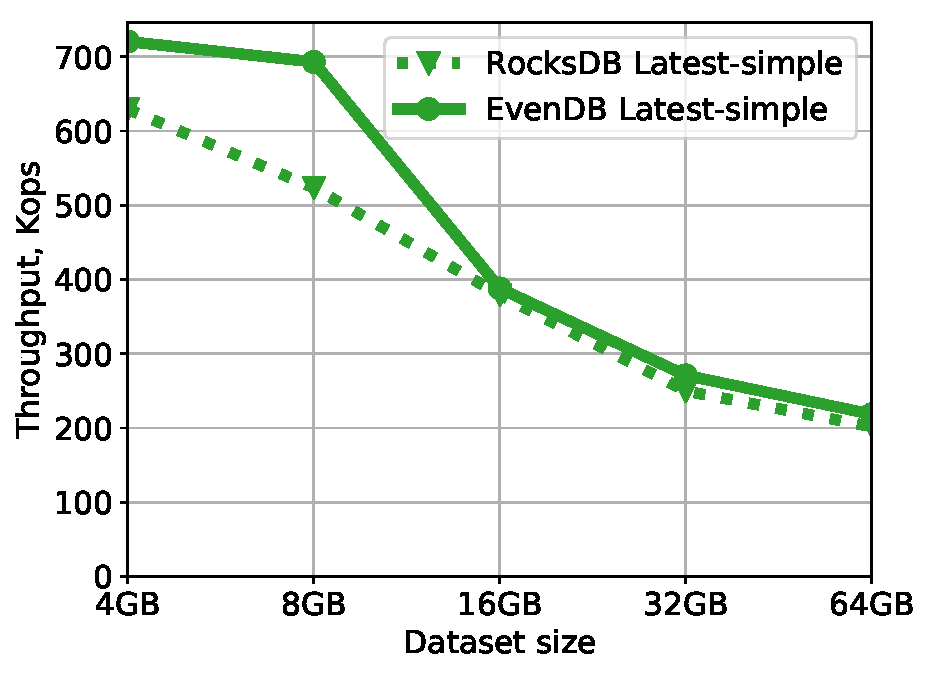
\includegraphics[width=\textwidth]{figs/Workload_D_line.pdf}
\caption{D -- Latest-simple, 5\% put, 95\% get}
\label{fig:throughput:d}
\end{subfigure}
\begin{subfigure}{0.33\linewidth}
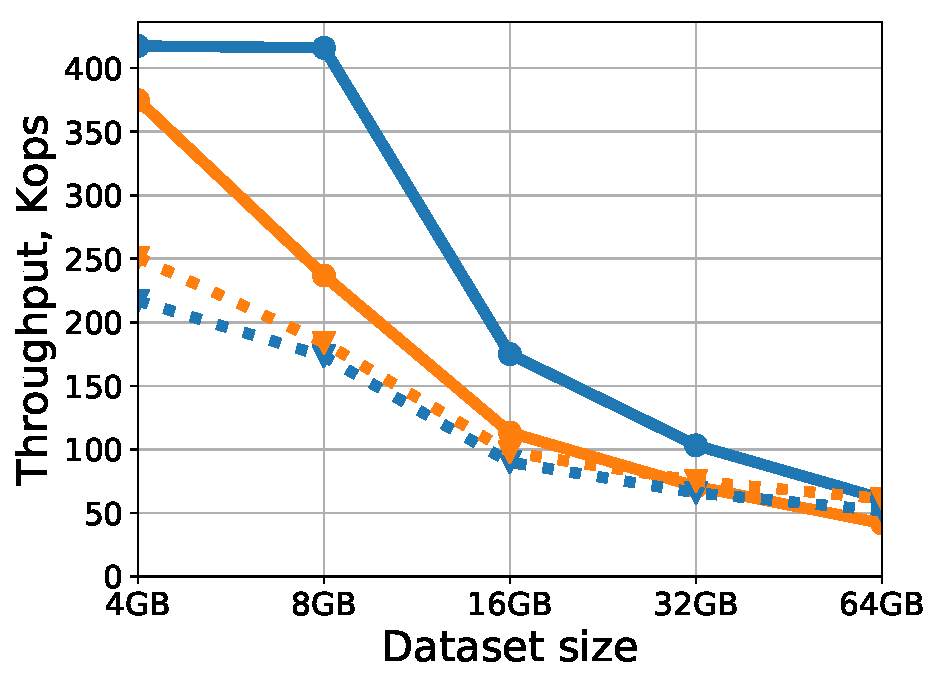
\includegraphics[width=\textwidth]{figs/Workload_F_line.pdf}
\caption{F -- 100\% get-modify-put}
\label{fig:throughput:f}
\end{subfigure}
\hspace{70pt}
\begin{subfigure}{0.33\linewidth}
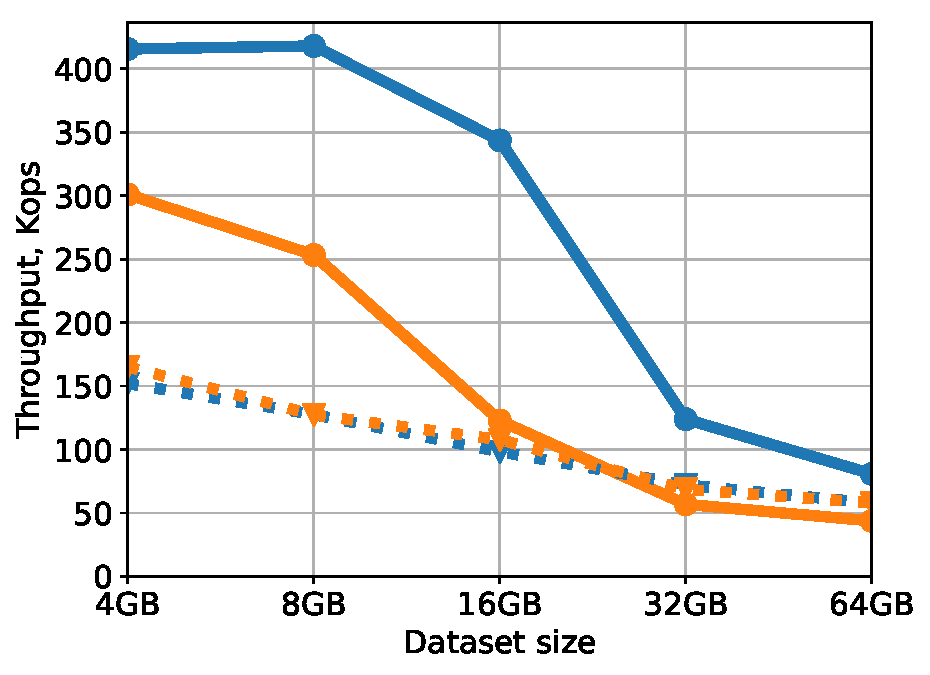
\includegraphics[width=\textwidth]{figs/Workload_E-_line.pdf}
\caption{E10 \\ 5\% put, 95\% scan (10 rows)}
\label{fig:throughput:e10}
\end{subfigure}
\begin{subfigure}{0.33\linewidth}
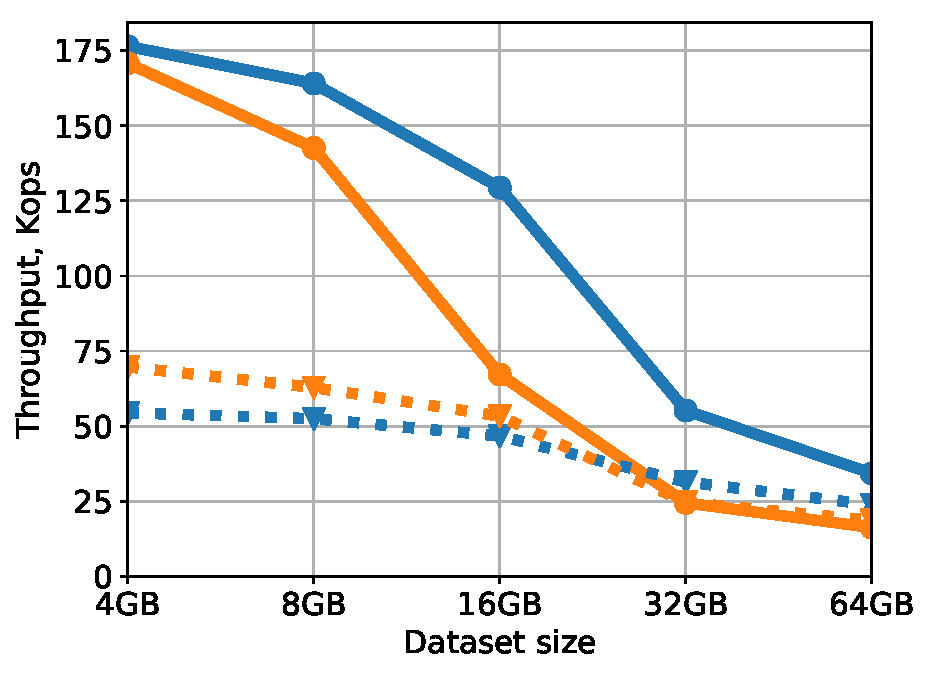
\includegraphics[width=\textwidth]{figs/Workload_E_line.pdf}
\caption{E100 \\ 5\% put, 95\% scan (100 rows)}
\label{fig:throughput:e100}
\end{subfigure}
\begin{subfigure}{0.33\linewidth}
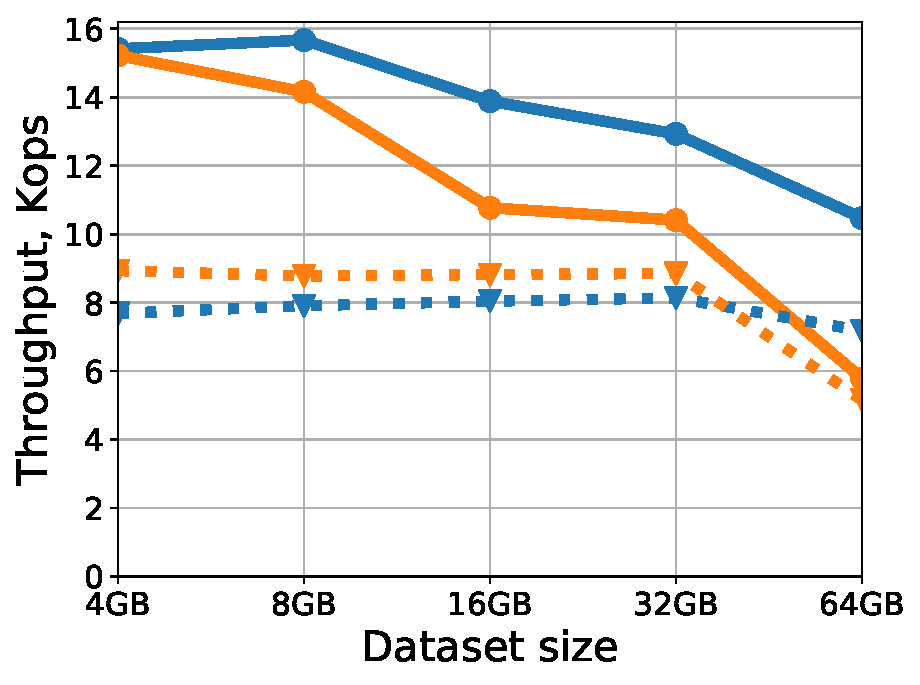
\includegraphics[width=\textwidth]{figs/Workload_E+_line.pdf}
\caption{E1000 \\5\% put, 95\% scan (1000 rows)}
\label{fig:throughput:e1000}
\end{subfigure}
\begin{subfigure}{\linewidth}
\centerline{

\includegraphics[width=0.9\textwidth]{figs/legend.pdf}
\vspace{-5mm}
}
\end{subfigure}
\caption{
{\sys\/ vs RocksDB throughput (Kops), under YCSB workloads with various key distributions.}
}
\label{fig:throughput}
\end{figure*}

We vary the dataset size from 4GB to 64GB in order to exercise multiple locality 
scenarios with respect to the available 16GB of RAM. Similarly to the published RocksDB benchmarks~\cite{RocksDBPerf}, 
the keys are 32-bit integers encoded in decimal form (10 bytes), which YCSB pads with a fixed 4-byte prefix (so effectively, 
the keys are 14 byte long). The values are 800-byte long. The data is stored uncompressed. 


Each experiment consists of three stages. The first stage populates the dataset by filling an initially empty store 
with a sequence of KV-pairs, ordered by key. 
The second phase is warm-up, running read-only operations to warm the caches. The third
phase exercises the specific scenario; all worker threads follow the same access pattern. We 
measure performance only during the steady state (skipping the load and warm-up phases). 
Most experiments  perform 80 million data accesses. Experiments with scans perform 4 to 16 million 
accesses, depending on the scan size. 

\subsubsection{Workloads}
%\paragraph{Workloads.} 


We study the following key-access distributions:  

%\begin{description}
%\item [Zipf-simple] 
\paragraph{Zipf-simple} -- the standard YCSB Zipfian distribution over simple (non-composite) keys. 
Key access frequencies are sampled from the heavy-tailed Zipf distribution 
following the description in~\cite{Gray:1994:QGB:191839.191886}, with $\theta = 0.8$. 
The ranking is over a random permutation of the entire key range, so popular keys are uniformly dispersed.
% The key locations are sampled uniformly at random from the whole data range. 
This workload exhibits medium temporal locality (e.g., the most popular key's frequency is approximately $0.7\%$)
and no spatial locality. 
%This is a standard YCSB workload that captures a multitude of use cases  -- e.g., a web page cache distribution by URL. 

%\item [Zipf-composite]  
\paragraph{Zipf-composite} -- a Zipfian distribution over composite keys. 
The key's $14$ most significant bits comprise the primary attribute. 
The primary attribute is drawn from a Zipf ($\theta=0.8$) distribution over its range. The remainder of the key is drawn uniformally at random.
We also experimented with a Zipfian distribution of the key's suffix; 
the performance trends were similar since performance is most affected by 
 the primary dimension's distribution. Zipf-composite exhibits high spatial locality.% it represents workloads 
%with composite keys.%, such as message threads~\cite{Borthakur:2011:AHG:1989323.1989438},
%social network associations~\cite{Armstrong:2013:LDB:2463676.2465296}, and analytics databases~\cite{flurry},
%and other scenarios with spatial locality of keys, e.g.,  reverse URL domains.

%\item [Latest-simple] 
\paragraph{Latest-simple} -- reading  recently added simple keys (e.g., status updates and reads). 
Keys are inserted in sequential  order; the read keys' distribution is skewed towards recently added ones. 
Specifically, the sampled key's position wrt the most recent key is distributed Zipf. This is a 
standard YCSB workload with medium spatial and temporal locality.

%\item [Uniform] 
\paragraph{Uniform} -- ingestion of keys in random order (the keys are sampled uniformly at random). RocksDB
reports a similar benchmark~\cite{rocksdb-benchmarks}; we present it for completeness.
%\end{description}

The workloads exercise different mixes of puts, gets, and scans. We use standard YCSB scenarios 
(A to F) that range from write-heavy ($50\%$ puts) to read-heavy ($95\%-100\%$ gets or scans). 
In order to stress the system even more on the write side, we introduce a new workload,  
P, comprised of $100\%$ puts; it captures a massive data ingestion scenario. 
%non-sequential data load scenario (e.g., an ETL from an external data pipeline~\cite{flurry}). 

\subsubsection{Evaluation results}
Figure~\ref{fig:throughput} presents throughput measurements of \sys\/ and RocksDB
in all YCSB workloads. Except workload D, which exercises the Latest-simple pattern
(depicted in green), all benchmarks are run with both  Zipf-simple (orange) 
and Zipf-composite (blue). The P (put-only) workload 
additionally exercises the Uniform access pattern (red). \sys\/ results are depicted with solid
lines, and RocksDB with dotted lines. 

We now discuss the results for the different scenarios.
  
\paragraph{ Put-only (data ingestion)} is tested in workload
{P} (100\% put, Figure~\ref{fig:throughput:p}). 
\sys's throughput is 1.8x to 6.4x that of RocksDB's with uniform keys, 1.3x to 2.3x with Zipf-composite keys, 
and 0.9x to 1.6x with Zipf-simple keys. This scenario's bottleneck is the reorganization of persistent data  
(funk rebalances in \sys, compactions in RocksDB), which causes write amplification and hampers performance. 
 
 Under the Zipf-composite workload, \sys\ benefits from spatial locality whereas RocksDB's write performance 
 is relatively insensitive to it, as is typical for LSM stores. For small datasets (4-8GB), \sys\/ accommodates 
all puts in munks, and so funk rebalances are rare. In big datasets, funk rebalances do occur, but mostly in 
munk-less chunks, which are accessed infrequently. This is thanks to \sys\/'s high log size limit for chunks 
with munks. Hence, in both cases, funk rebalances incur less I/O than RocksDB's compactions, 
which do not distinguish between hot and cold data. Note that \sys's recovery time is not impacted by 
long funk logs since they are not replayed upon recovery.

 Under the Zipf-simple workload, the gains are moderate due to the low spatial locality. They are most pronounced 
 for small datasets that fit into RAM.
 
The Uniform workload exhibits no locality of any kind. 
 \sys\/ benefits from this because the keys get dispersed evenly across all chunks, hence all funk logs grow 
 slowly, and funk rebalances are infrequent. The throughput is therefore insensitive to the dataset 
 size. In contrast, RocksDB performs compactions frequently albeit they are not effective (since there are few redundancies). Its throughput 
 degrades  with the data size since when compactions cover more keys they engage more files.
 
 \remove{
 \inred{Increasing RocksDB's block cache size to 5GB is counterproductive in this scenario because it steals 
 resources from the write path (e.g., reducing the throughput by 0.33x for the 64GB dataset under Zipf-simple).}
 }
   
The write amplification in this experiment is summarized in 
Figure~\ref{fig:writeamp}. We see that \sys\/ reduces the disk write rate dramatically, 
with the largest gain observed for big datasets (e.g.,  for the 64GB dataset 
the amplification factors are $1.3$ vs $3.1$ under Zipf-composite, and $1.1$ vs $7.6$ under Uniform). 
%Thus, \sys\/ also reduces disk wear in multiple scenarios. 
%\inred{It should be noted that \sys\/'s low write amplification on the Uniform distribution would have increased on longer runs, as logs fill up and invoke funk rebalances. However, longer runs would have also caused larger RocksDB rebalances.}

%\begin{table}[t]
%\centerline{
%{\small{
%\begin{tabular}{lccccc}
%\hline 
% & 4GB & 8GB & 16GB & 32GB & 64GB \\
%\hline 
%Zipf-composite: &  \multicolumn{5}{c}{}  \\
%RocksDB & 2.08	& 2.29 & 2.35 & 2.40	& {\bf {3.10}}\\
%\sys &  1.33	 & 1.30	& 1.22	& 1.25	& { {\bf 1.34}}\\
%\hline 
%Zipf-simple: &  \multicolumn{5}{c}{}   \\
%RocksDB & 1.92	& 1.95 & 2.02 & 2.20	& 2.44 \\
%\sys &  1.31	 & 1.27	& 1.08	& 1.20	& 1.19 \\
%\hline 
%Uniform: &  \multicolumn{5}{c}{}   \\
%RocksDB & 1.92	& 1.95 & 2.02 & 2.20	& 2.44 \\
%\sys &  1.31	 & 1.27	& 1.08	& 1.20	& 1.19 \\
%\hline 
%\end{tabular}
%}}
%}
%\caption{{\sys\/ versus RocksDB write amplification under the put-only workload P.}}
%\label{fig:writeamp}
%\end{table}

\begin{figure}[t]
	\centering
	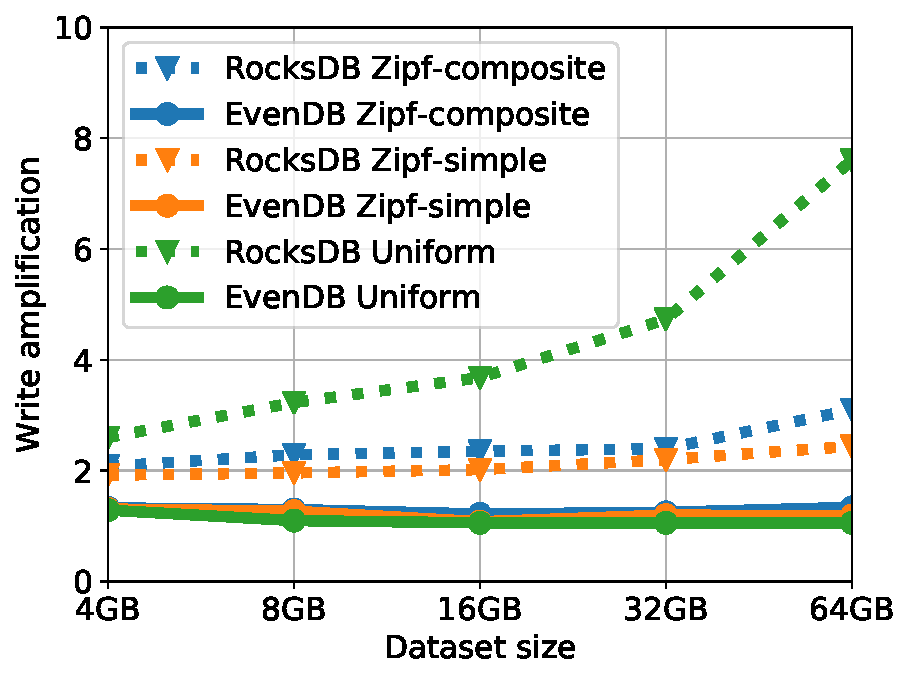
\includegraphics[width=0.35\textwidth]{figs/write_amp_p_line.pdf}
	\caption{{\sys\/ vs RocksDB write amplification under the put-only workload P.}}
	\label{fig:writeamp}
\end{figure}

\remove{
\inred{
\sys\/ advantages are also evident when puts are uniformly distributed (green lines in Figure~\ref{fig:throughput:p}). Since funk rebalances are local, the distribution of rebalances (dictated by the distribution of puts) has little effect. In RocksDB, however, each L0 SST contains keys covering a wide range of keys, causing L0 to L1 compactions to include a large number of SSTs.
}}

\paragraph{ Mixed put-get} is represented in workloads A (50\% put, 50\% get, Figure~\ref{fig:throughput:a}) and 
F (100\% get-modify-put, Figure~\ref{fig:throughput:f}). Note that the latter exercises the usual get and put API (i.e., does not provide atomicity). 
In this scenario, \sys\ works well with composite keys, e.g., in workload A it  achieves $1.4$x to $3.5$x the throughput of RocksDB due to better exploitation of spatial locality. 
With simple keys, on the other hand, the get-put mix is particularly challenging for \sys, which serves many gets from disk due to the
low spatial locality. The bottleneck is the linear search in funk logs, which  fill
up due to the high put rate.
RocksDB's caching is more effective in this scenario, so its disk-access rate in get operations is lower,  resulting in faster gets. 
Note that \sys\/ is still reasonably close to RocksDB in the worst case 
(0.75x and 0.7x throughput for the 64GB dataset in A and F, respectively).
%(In-memory searches are three orders of magnitude faster.)

Figure~\ref{fig:tail_latency}, which depicts tail (95\%) put and get latencies in this scenario, 
corroborates our analysis. \sys\/ has faster puts and faster or similar get tail latencies with composite keys
(Figure~\ref{fig:tail_latency:co}). With simple keys (Figure~\ref{fig:tail_latency:si}),  
the tail put latencies are similar in the two data stores, but the tail get latency of \sys\ 
in large datasets surges.

 To understand this spike, 
we break down the get latency in  Figure~\ref{fig:readstat}. 
Figure~\ref{fig:readstat:dist} classifies gets by the storage  component 
that fulfills the request, and Figure~\ref{fig:readstat:lat} presents the disk search latencies by component. 
We see that with large datasets, disk access dominates the latency.
For example, in the 64GB dataset, $3.3\%$ of gets are served from logs under Zipf-composite, vs $4.0\%$ under Zipf-simple,
and the respective log search latencies are $2.6$ ms vs $4.2$ ms. This is presumably because in the latter, puts are more dispersed, 
hence the funks are cached less effectively by the OS, and the disk becomes a bottleneck due to the higher I/O rate.
%and (2) rebalanced less frequently so their logs grow longer.

\remove{
\begin{figure*}[tb]
\centering
\begin{subfigure}{0.36\linewidth}
\vskip .15in
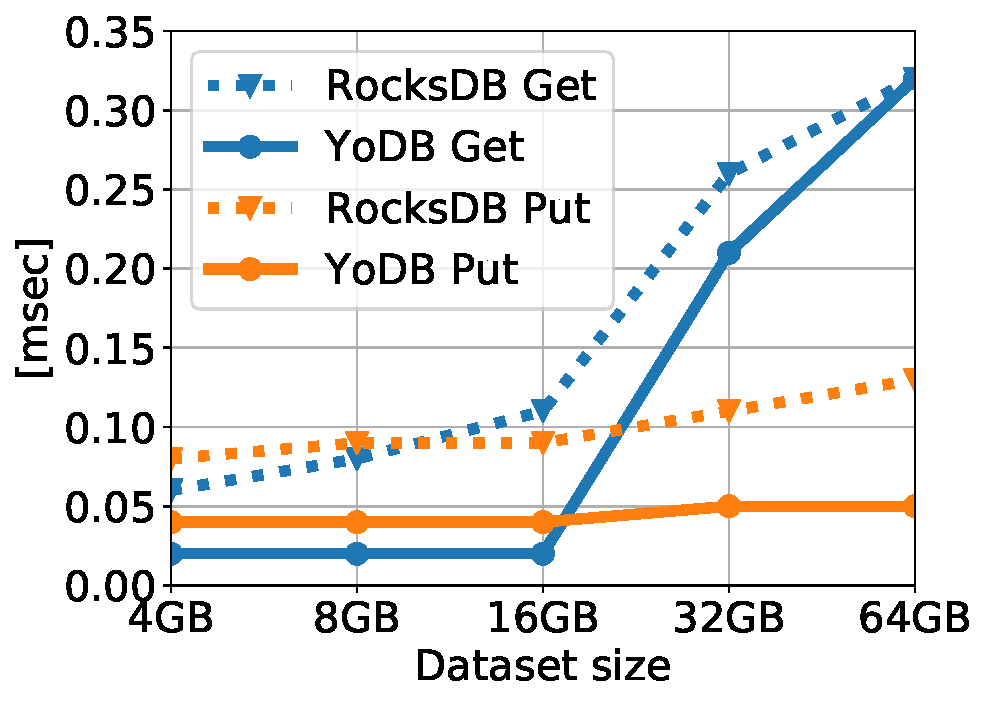
\includegraphics[width=\textwidth]{figs/tail_line.pdf}
\vskip .55in
\caption{95-percentile latency, put and get}
\label{fig:tail_latency:lat}
\end{subfigure}
\begin{subfigure}{0.32\linewidth}
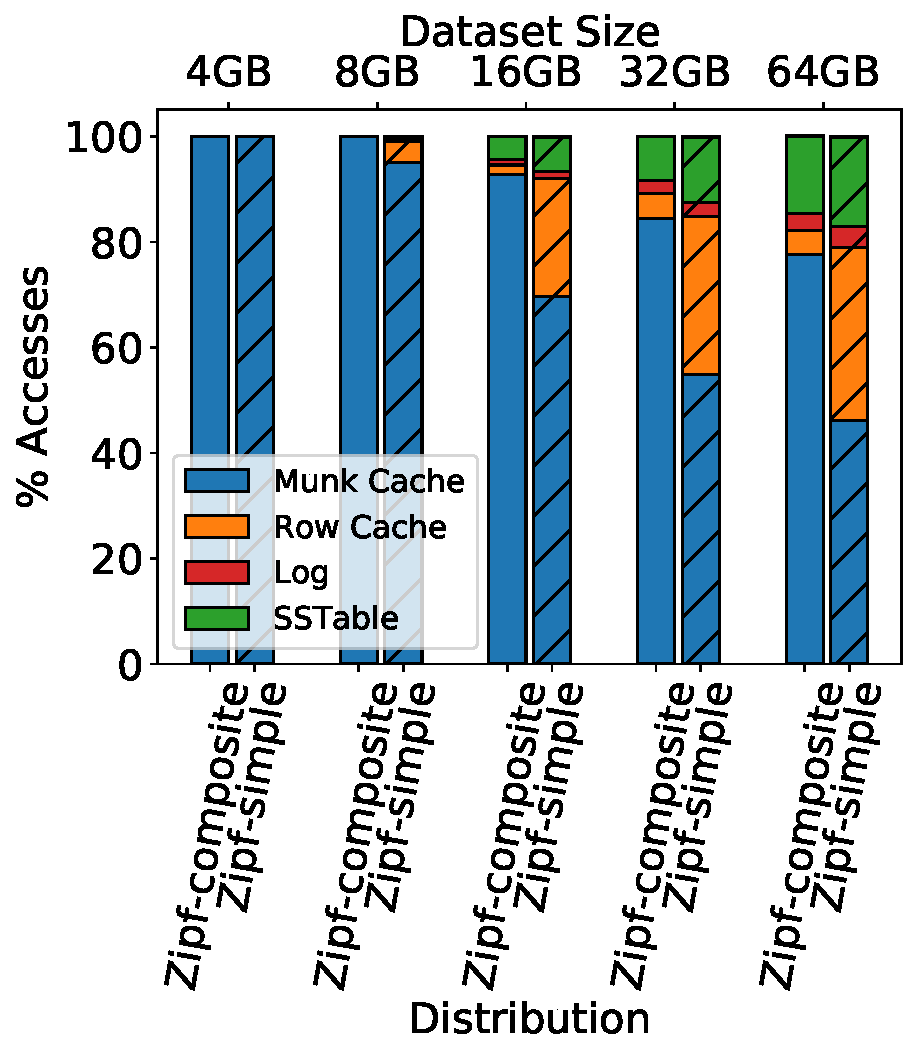
\includegraphics[width=\textwidth]{figs/Time_percentage_A.pdf}
\caption{Fraction of get accesses, by component}
\label{fig:tail_latency:dist}
\end{subfigure}
\begin{subfigure}{0.31\linewidth}
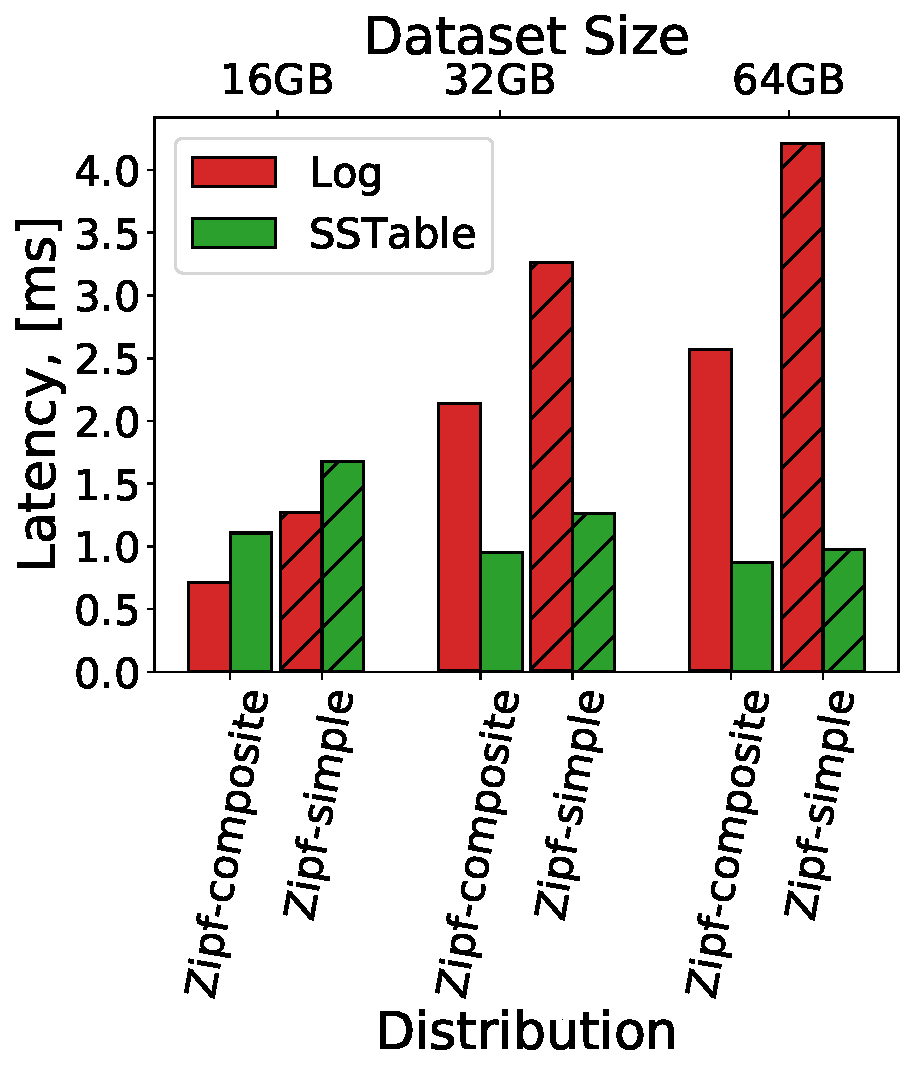
\includegraphics[width=\textwidth]{figs/Latency_A.pdf}
\caption{On-disk get latency, by component}
\label{fig:tail_latency:disk}
\end{subfigure}
\label{fig:tail_latency}
\caption{{\sys\/ tail latency analysis, under a mixed get-put workload A.}}
\end{figure*}
}

\begin{figure}[htb]
\centering
\begin{subfigure}{0.49\linewidth}
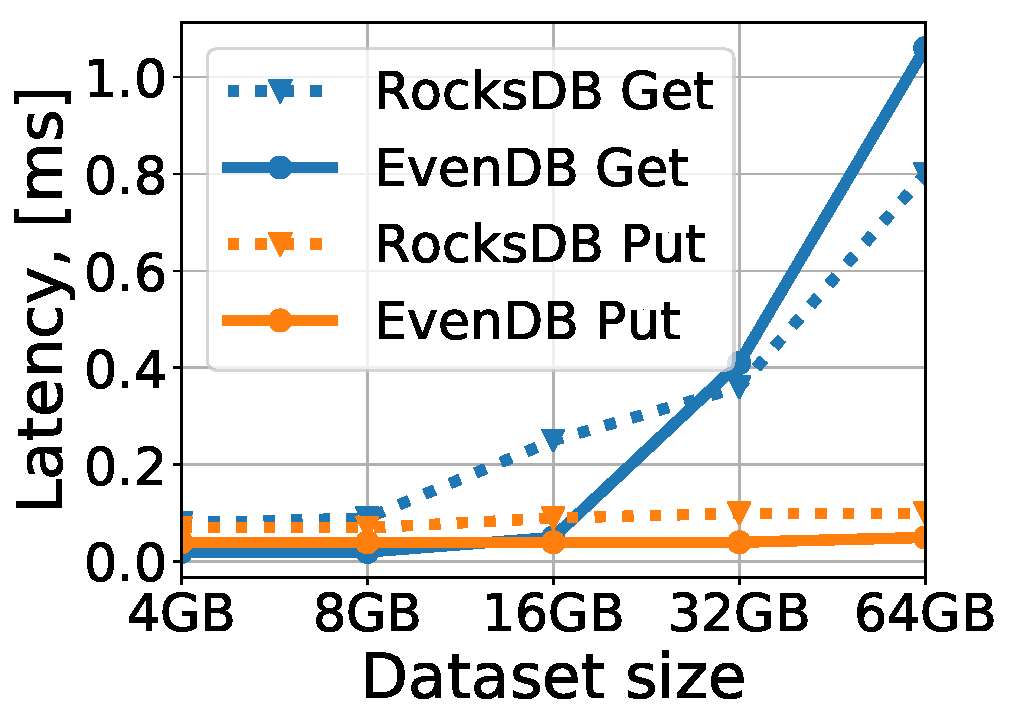
\includegraphics[width=\textwidth]{figs/tail_flurry_line.pdf}
\caption{Zipf-composite}
\label{fig:tail_latency:co}
\end{subfigure}
\begin{subfigure}{0.49\linewidth}
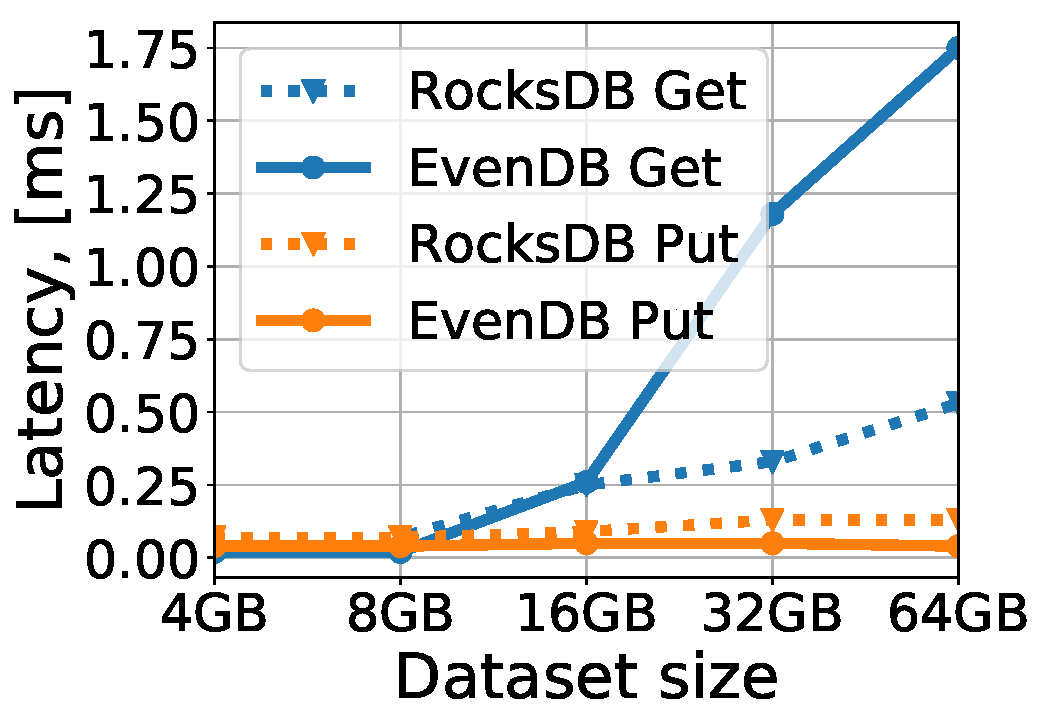
\includegraphics[width=\textwidth]{figs/tail_zipf_line.pdf}
\caption{Zipf-simple}
\label{fig:tail_latency:si}
\end{subfigure}
\caption{{\sys\/ vs RocksDB 95\% latency (ms), under a mixed get-put workload A.}}
\label{fig:tail_latency}
\end{figure}

\begin{figure}[htb]
\centering
%\hspace{0.05\linewidth}
\begin{subfigure}{0.5\linewidth}
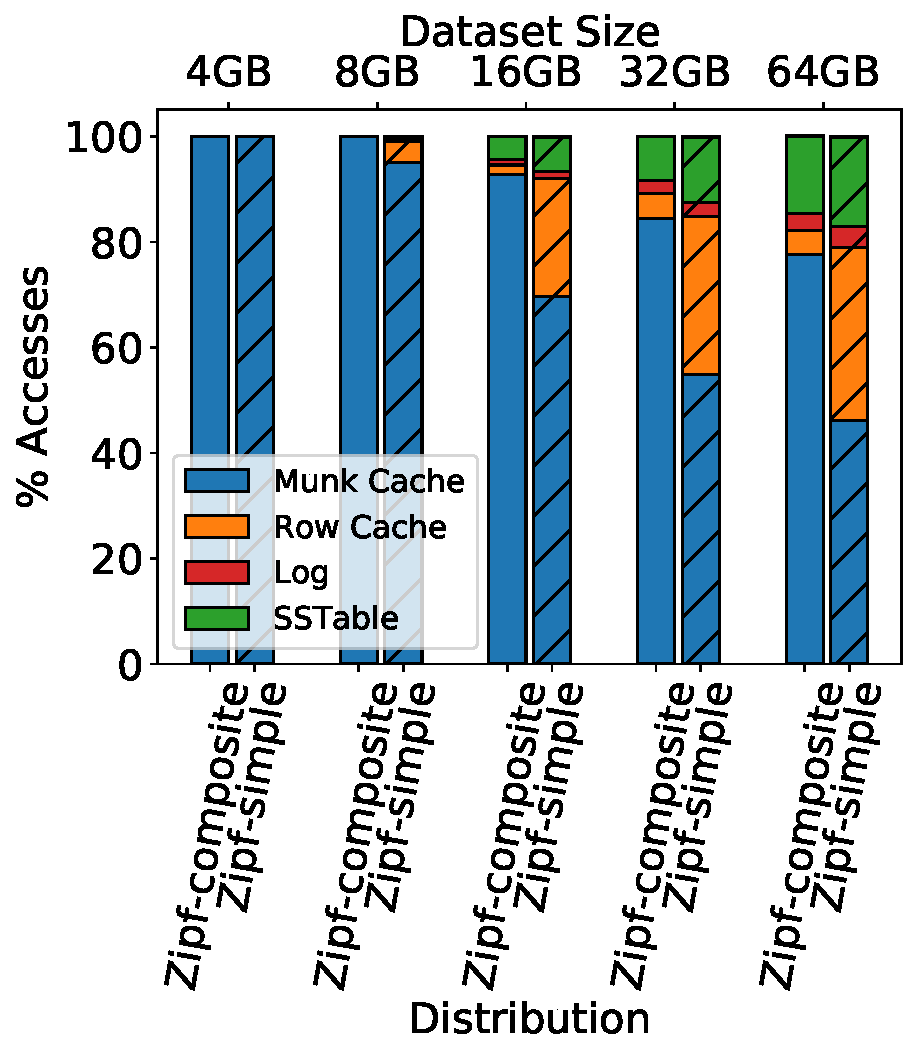
\includegraphics[width=\textwidth]{figs/Time_percentage_A.pdf}
\vskip .1in
\caption{Fraction of get accesses}
\label{fig:readstat:dist}
\end{subfigure}
%\hspace{0.05\linewidth}
\begin{subfigure}{0.49\linewidth}
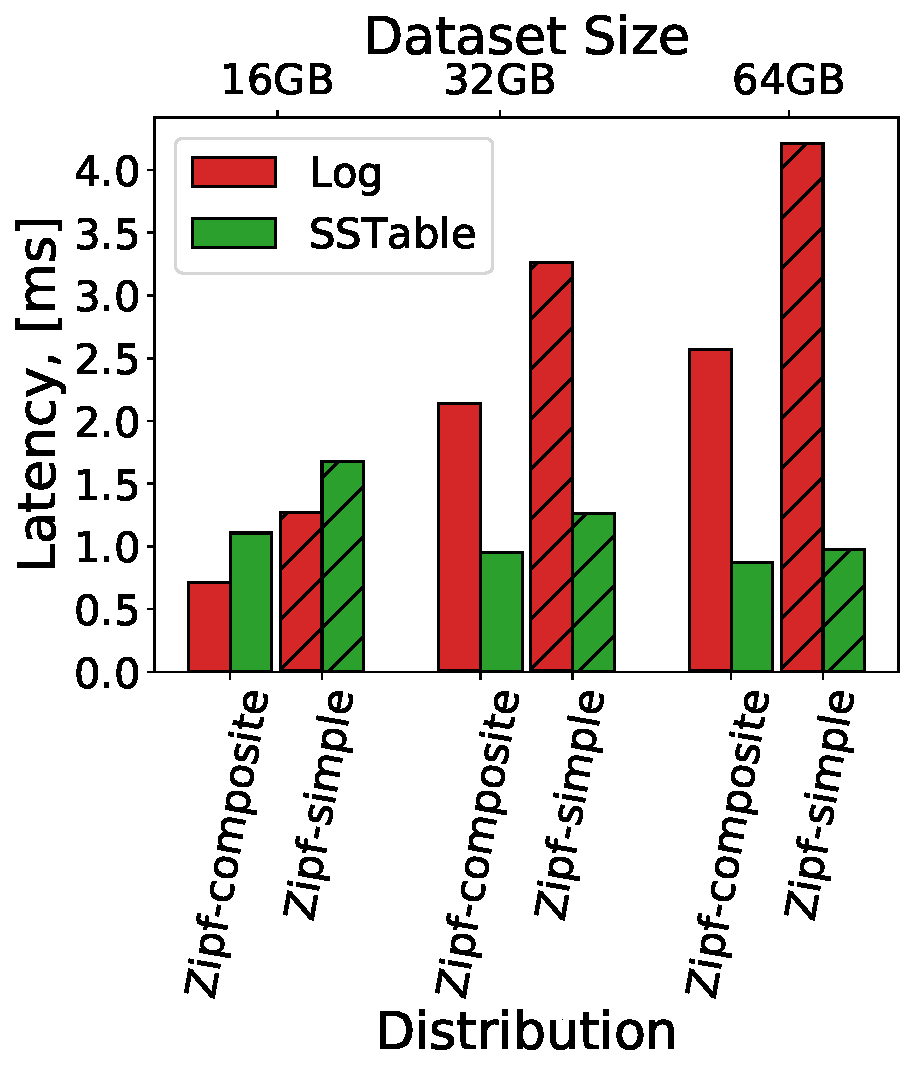
\includegraphics[width=\textwidth]{figs/Latency_A.pdf}
\caption{On-disk get access latency}
\label{fig:readstat:lat}
\end{subfigure}
\caption{{\sys\/ get latency breakdown by serving component, under a mixed get-put workload A.}}
\label{fig:readstat}
\end{figure}

%In-memory caching is paramount. In the same case, the RAM hit rate 
%(munks and row cache combined) is $82.1\%$ with composite keys vs. $79\%$ without them. 
The figure also shows that the row cache becomes instrumental as spatial locality drops -- it serves $32.8\%$ of gets with Zipf-simple 
vs $4.5\%$ with Zipf-composite. 

\paragraph{ Get-dominated} 
workloads (B--D, Figures~\ref{fig:throughput:b}--\ref{fig:throughput:d}) are 
favorable to 
\sys, which has a marked advantage in all key distributions with small datasets (up to the available RAM size) 
and also with Zipf-composite keys in large datasets. 
For example, in workload C (100\% get, Figure~\ref{fig:throughput:c}), 
\sys\/ performs $1.2$x to $2$x better than RocksDB with composite keys,
and up to $1.9$x  with simple ones (for small datasets). 
In these scenarios, \sys\  manages to satisfy most gets from munks, resulting in good performance.
RocksDB relies mostly on the OS cache to serve these requests and so it pays the overhead for invoking system calls. 
As we discuss in~\S\ref{ssec:drill} below, 
RocksDB's performance in this scenario can be improved by using a larger application-level block cache,
but this hurts performance in other benchmarks.

\paragraph{ Scan-dominated} benchmarks (E10--1000,  5\% put, 95\% scan, Figures~\ref{fig:throughput:e10}-~\ref{fig:throughput:e1000})
iterate through a number of items 
sampled uniformly in the range [1,S], where S is  10, 100, or 1000. 
This workload (except with short scans on  large datasets) is favorable to \sys, 
since it exhibits the spatial locality the system has been designed for. 
Under Zipf-composite, \sys\/ achieves $1.4$x to $3.2$x throughput vs RocksDB.   
With simple keys, \sys\ improves over RocksDB when scans are long or the dataset is small. 
In \S\ref{ssec:drill} we show that \sys's scan performance on big datasets can be improved by adapting the 
funk log size limit to this workload. 
%(The experiments reported herein all use the default configuration).
 
\remove{
Note that the scan speed is  higher for the 8GB dataset vs the 4GB dataset. 
Both are quite fast as they are served from memory, but in the smaller dataset there is more contention 
between scans and puts, which slows down   progress. }
%This phenomenon becomes insignificant with longer scans. 

\remove{

\inred{TODO. Zipf-composite reaches 1.2x-2.4x, while zipf-simple starts with 1.5x on 4GB DB, but degrades to 0.7x on 64GB DB. This is the results of an update rate like in A, combined with 100\% read rate. The RMW implementation here was at the YCSB level, hence identical for RocksDB and \sys\/. RocksDB does have a native RMW primitive that works differently (a modification predicate is stored, moving actual computation to gets). \sys\/ doesn't have such a primitive, making the workload less indicative.}

Since workload C only exercises the read path, performance hinges on 
caching efficiency. Both \sys\ and RocksDB benefit from  OS (filesystem) caching in addition to application-level caches. 
Table~\ref{fig:readamp} compares the two systems' read amplification (as a proxy for cache hit ratio) with composite keys, 
in terms of (1) actual disk bytes read and (2) read system calls.  Under the first, 
RocksDB is slightly better in large datasets. However, it relies extensively on the OS cache -- in the 64GB dataset, 
%, at the expense of the user-level block cache. In the same setting, 
it performs almost 12 times as many system calls as \sys,  wasting the CPU resources on  
kernel-to-user data copy. RocksDB developers explain that the block cache scaling potential is limited in their
database, due to tension between its read-path and write-path RAM resources~\cite{RocksDB-default-blockcache-issue}. 
\sys, in contrast, exploits its munk cache for both reads and writes, which leads to better RAM utilization. 


\begin{table}[htb]
{\small{
\begin{tabular}{lccccc}
\hline 
& 4GB & 8GB & 16GB & 32GB & 64GB \\
\hline 
RocksDB, bytes &  0.05 &	0.11 & 0.20 & 0.47 & 0.95\\
\sys, bytes &  0.0 &	0.0 &	0.11	& 0.80	& 1.07 \\
\hline 
RocksDB, syscall & 3.84	& 4.01	& 4.14	& 4.28	& {\bf {4.37}} \\ 
\sys, syscall  & 0.0 & 0.0	& 0.10 & 0.24 & {\bf {0.41}} \\
\hline 
\end{tabular}
}}
\caption{{\sys\/ vs RocksDB read amplification, in terms of bytes and system calls, 
under a read-only workload C with Zipf-composite distribution.}}
\label{fig:readamp}
\end{table}
}


\remove{
\begin{figure}[t]
\centering
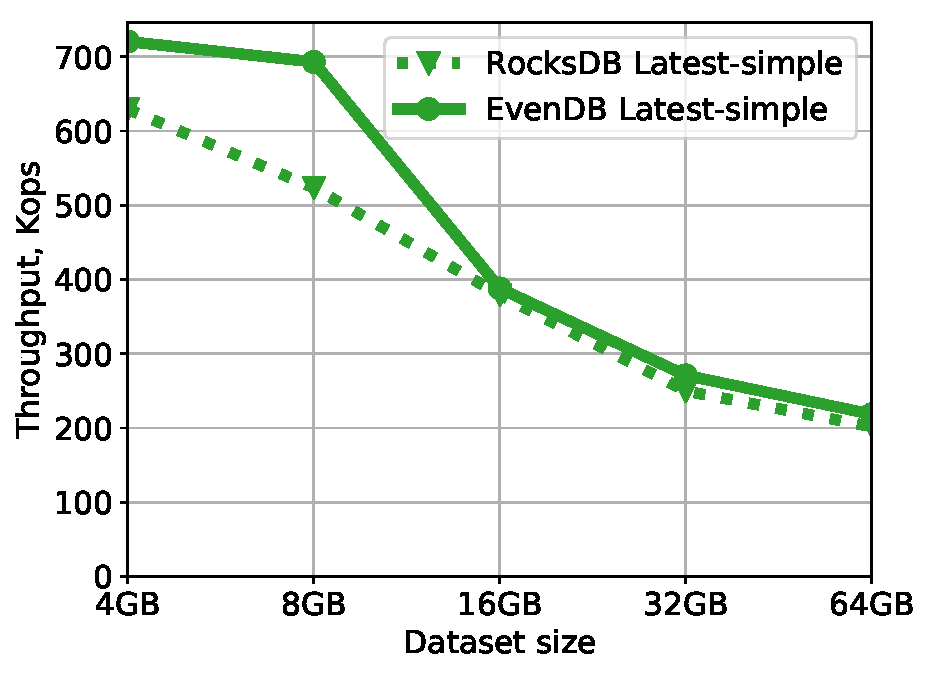
\includegraphics[width=0.4\textwidth]{figs/Workload_D_line.pdf}
\caption{{\sys\/ vs RocksDB throughput, under the D workload.}}
\label{fig:throughput:d}
\end{figure}
}

\subsection{Insights}
\label{ssec:drill} 

\paragraph{Vertical scalability.} 
Figure~\ref{fig:scalability} illustrates \sys's throughput scaling for the 64GB dataset under Zipf-composite and Zipf-simple  
distributions. We exercise the A, C and P scenarios, with 1 to 12 worker threads.  
As expected, in C (100\% gets) \sys\/ scales nearly perfectly (7.7x for composite keys, 7.8x for simple ones). 
The other workloads scale slower, due to read-write and write-write contention as well as background munk and funk rebalances. 
%P scales 3.8x for both distributions at 8 threads. A scales 6.4x for Zipf-composite and 4.6x for Zipf-simple at 12 threads. 

\begin{figure}[th]
\centering
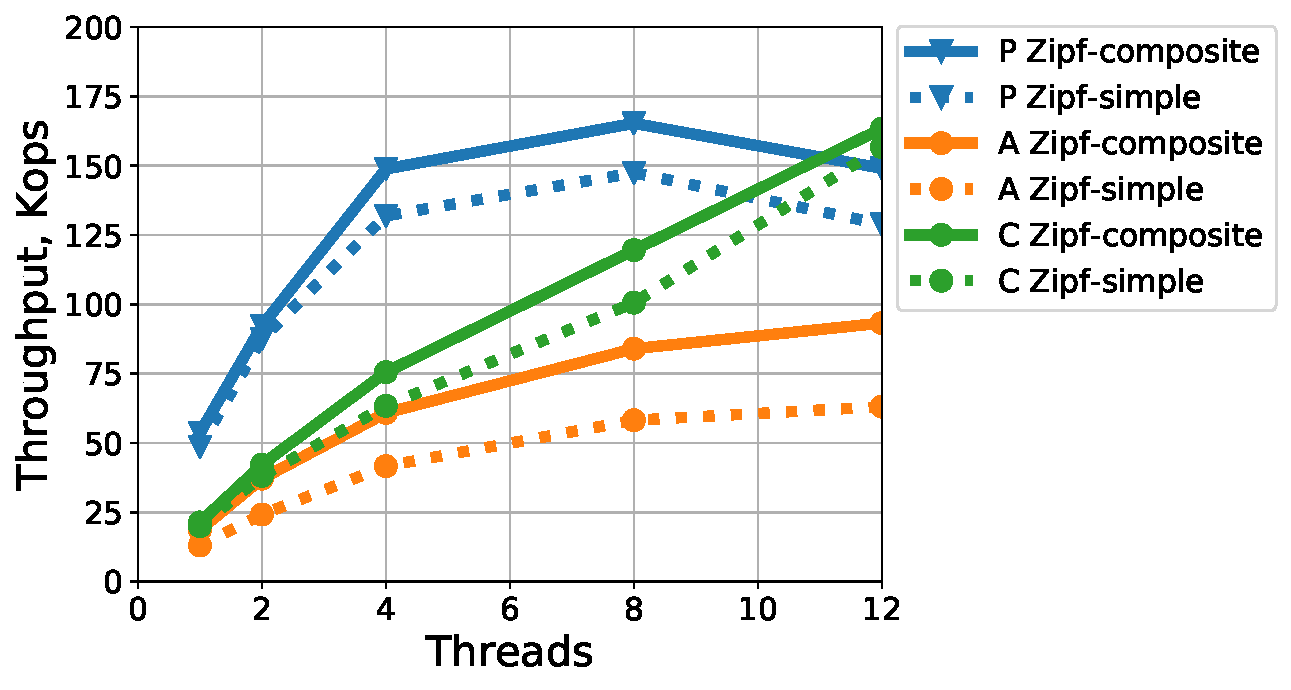
\includegraphics[width=0.4\textwidth]{figs/scalability_line.pdf}

\caption{{\sys\/ scalability with the number of threads for 
the 64GB dataset and different workloads. }}
\label{fig:scalability}
\end{figure}

\remove{
\begin{table*}
\centering
%\begin{subfigure}{0.55\linewidth}
{\small{
\begin{tabular}{l|cccccc|c|ccccc|}
\cline{2-7} \cline{9-13} 
  & \multicolumn{6}{c|}{Maximum log size} & & \multicolumn{5}{c|}{Bloom filter split factor}\\
%\cline{2-7} \cline{9-13} 
& 128KB & 256KB & 512KB & 1MB & 2MB & 4MB & &1 & 2 & 4 & 8 & 16 \\
\cline{2-7} \cline{9-13} 
Zipf-composite: & 50.2	& 55.5 & 80.7	& 134.1 & {\bf {157.5}} & 149.5 & & 134.7 & 133.5 & 140.1 & 152.5 & {\bf {157.4}}   \\
Zipf-simple:    & 27.8	& 30.9 & 36.1	& 58.3  & {\bf {68.3}}   & 68.1   & &  36.3 & 39.2   & 46.3  & 56.0  & {\bf {59.9}}\\
%\hline 
%E, Zipf-range & 29.1	& 36.4 & 36.9	& 37.3	& {\inred{30.4}} & 	37.1 \\
%E, Zipf & 16.1 & 16.3 &	15.8	& 15.8 &	16.4 &	15.8 \\
\cline{2-7} \cline{9-13} 
\end{tabular}
}}
%\caption{Throughput (Kops) vs log size}
%\label{fig:wal:sz}
%\end{subfigure}
%\hspace{0.09\linewidth}
%\begin{subfigure}{0.35\linewidth}
%{\small{
%\begin{tabular}{|l|c|c|c|c|}
%\hline 
%1 & 2 & 4 & 8 & 16\\
%\hline 
%134.7 & 133.5 & 140.1 & 152.5 & {\bf {157.4}} \\
% 36.3 & 39.2 & 46.3 & 56.0 & {\bf {59.9}} \\
%\hline 
%\end{tabular}
%}}
%\caption{Throughput (Kops) vs Bloom filter split factor}
%\label{fig:wal:bf}
%\end{subfigure}
\caption{{\sys\/ throughput under a mixed get-put workload A, 64GB dataset, and different configuration parameters.}}
\label{fig:wal}
\end{table*}
}

\begin{figure}[htb]
\centering
\begin{subfigure}{0.49\linewidth}
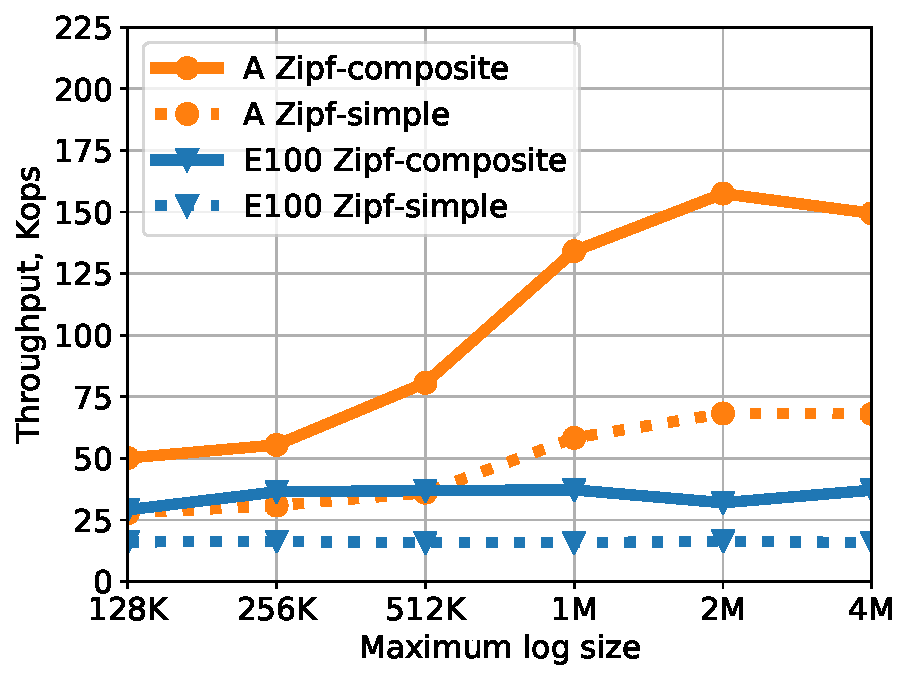
\includegraphics[width=\textwidth]{figs/max_log_size_line.pdf}
\caption{Maximum log size,\\  workloads A and E100}
\label{fig:params:log}
\end{subfigure}
%\hspace{0.05\linewidth}
\begin{subfigure}{0.49\linewidth}
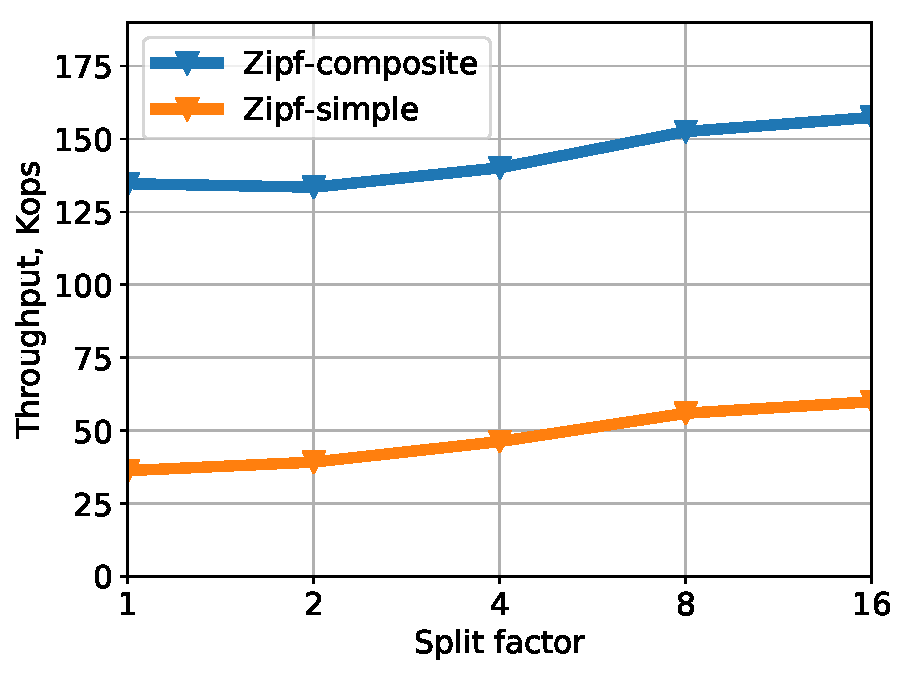
\includegraphics[width=\textwidth]{figs/Bloom_filter_line.pdf}
\caption{Bloom filter split factor,\\ workload A}
\label{fig:params:bf}
\end{subfigure}
\caption{{\sys\/ throughput sensitivity to configuration parameters, on the 64GB dataset under  A (mixed put-get) and 
E100 (scan-dominant, 1 to 100 items).}}
\label{fig:params}
\end{figure}

\paragraph{\sys\/ configuration parameters.} 
We explore the system's  sensitivity to funk-log configuration parameters, for the most challenging 64GB dataset, 
and explain the choice of the default values.

Figure~\ref{fig:params:log} depicts the throughput's dependency on the log size limit of munk-less funks, 
under  A and E100  with the Zipf-composite key distribution. 
The fraction of puts in A is 50\% (vs 5\% in E), which makes it more sensitive to the log size. 
A low threshold (e.g., 128KB) causes frequent funk rebalances, which degrades performance more than 3-fold. 
On the other hand, too high a threshold (4MB) lets the logs grow bigger, and slows down gets. Our experiments  
use 2MB logs, which favors write-intensive workloads. E favors smaller logs, since the write 
rate is low, and more funk rebalances can be accommodated. Its throughput can  grow by up to 20\% 
by tuning the system to use 512KB logs.

Figure~\ref{fig:params:bf} depicts the throughput dependency on the Bloom filter split factor (i.e., the 
number of Bloom filters that summarize separate portions of the funk log) in workload A. 
Partitioning to 16 mini-filters gives the best result; \inred{Idit: the following was not shown: beyond this point the benefit levels off}. 
The impact of Bloom filter partitioning on \sys's %end-to-end get latency as well as the 
memory footprint is negligible.

\paragraph{RocksDB memory tuning.} In RocksDB's out-of-the-box default configuration, the block cache is 8MB. 
We next experiment with block cache sizes of 1GB, 2GB, 5GB, and 8GB. We note that 
RocksDB's performance manual recommends allocating 1/3 of the available RAM 
($\sim$5GB) to the block cache~\cite{RocksDBMemoryTuning}.
The results are mixed. For a small 
dataset (4GB) with composite keys, the block cache effectively replaces 
the OS pagecache, and improves RocksDB's throughput by $1.3$x and 1.6x
for workloads C and E100, respectively, by forgoing the system call overhead. This only partly reduces the gap between
RocksDB and \sys\/ in this setting. 

\begin{figure}[htb]
\inred{Eran please add a graph}
\caption{RocksDB's speedup with larger block caches than its default configuration. Results below $1$ indicate slowdown.}
\label{fig:rocks-memory}
\end{figure}

However, for  bigger datasets (32GB and 64GB),   using a  bigger 
block cache degrades  RocksDB's performance. Figure~\ref{fig:rocks-memory} shows 
RocksDB's speedup with different block cache sizes for the 64GB dataset in the various workloads. 
We see that the default configuration gives the best results for most of the workload suite (i.e., the 
speedups are mostly below $1$). We therefore used this configuration  in~\S\ref{ssec:synthetic} above.   

\subsection{\sys\ versus PebblesDB}
\label{ssec:pebbles} 

We compare \sys\ to PebblesDB, which was shown to significantly improve over RocksDB~\cite{PebblesDB},
mostly in single-thread experiments, before RocksDB's recent version was released.  
We compare \sys\ to PebbelesDB in a challenging  scenario for \sys, with a 32GB dataset and the Zipf-simple key 
distribution. We run each YCSB workload with 1, 2, 4, and 8 threads. The results are summarized in Table~\ref{fig:pebbels-throughput}. 
In all experiments, \sys\ is consistently better than PebblesDB, with its performance improvements ranging from \inred{1.5x} with a single thread
on P, to \inred{4.5x} with eight threads on E10.  In all benchmarks, 
 \sys's advantage grows with the level of parallelism. 
\inred{  
We observed a similar trend with smaller datasets. 
Idit: can we say more?
}

We note that in our experiments, RocksDB also consistently outperforms PebblesDB. 
The gap with the results reported in~\cite{PebblesDB} 
can be attributed, e.g., to RocksDB's evolution, resource constraints (running within a 
container), different hardware, and increased benchmark parallelism.   

\begin{table}
\centering
{\small{
\begin{tabular}{ccccccc}
%Workload & Zipf-simple & Zipf-composite \\
P & A & B & C & D& E10--1000 & F \\
\hline 
1.5--2.9x & \inred{TBD} & \inred{TBD} & 2.1--3.2x &  \inred{TBD} & 2.2--4.5x &  \inred{TBD}  \\
\end{tabular}
}}
\caption{{\sys\/ throughput improvement over PebblesDB, on a 32GB dataset with Zipf-simple keys, with 1 to 8 threads.}}
\label{fig:pebbels-throughput}
\end{table}




  